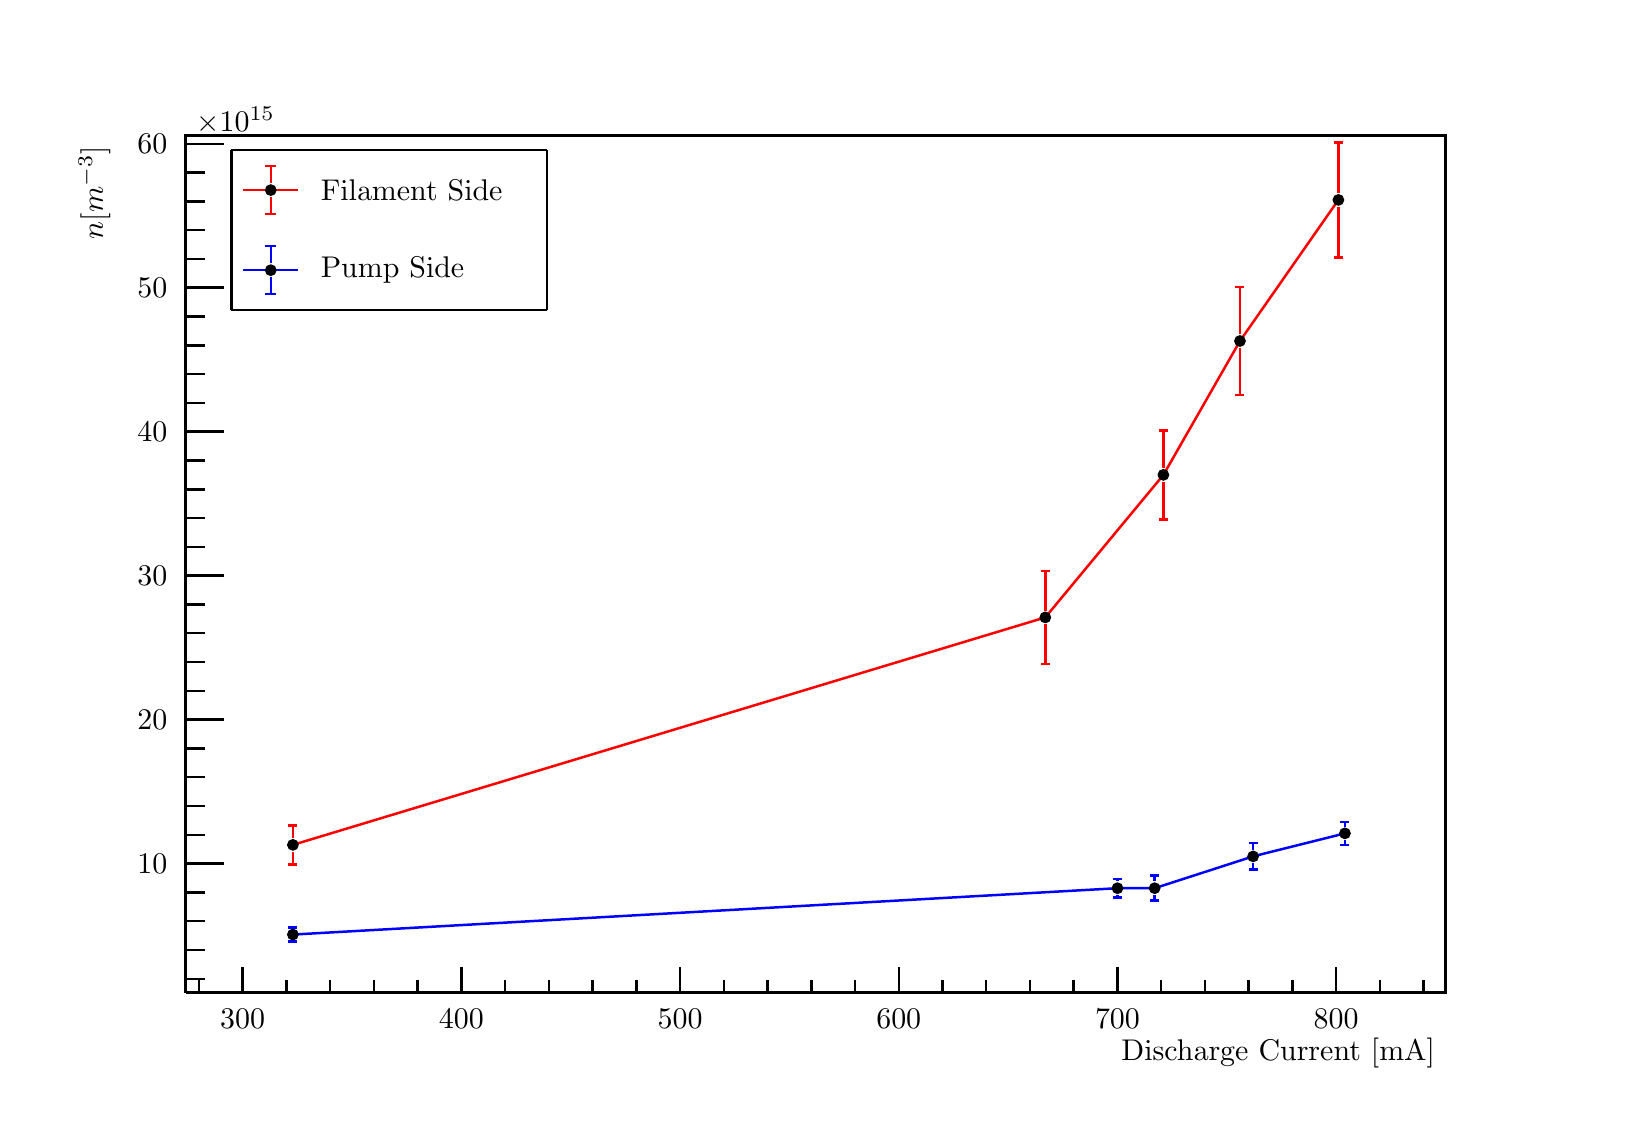
\begin{tikzpicture}
\pgfdeclareplotmark{cross} {
\pgfpathmoveto{\pgfpoint{-0.3\pgfplotmarksize}{\pgfplotmarksize}}
\pgfpathlineto{\pgfpoint{+0.3\pgfplotmarksize}{\pgfplotmarksize}}
\pgfpathlineto{\pgfpoint{+0.3\pgfplotmarksize}{0.3\pgfplotmarksize}}
\pgfpathlineto{\pgfpoint{+1\pgfplotmarksize}{0.3\pgfplotmarksize}}
\pgfpathlineto{\pgfpoint{+1\pgfplotmarksize}{-0.3\pgfplotmarksize}}
\pgfpathlineto{\pgfpoint{+0.3\pgfplotmarksize}{-0.3\pgfplotmarksize}}
\pgfpathlineto{\pgfpoint{+0.3\pgfplotmarksize}{-1.\pgfplotmarksize}}
\pgfpathlineto{\pgfpoint{-0.3\pgfplotmarksize}{-1.\pgfplotmarksize}}
\pgfpathlineto{\pgfpoint{-0.3\pgfplotmarksize}{-0.3\pgfplotmarksize}}
\pgfpathlineto{\pgfpoint{-1.\pgfplotmarksize}{-0.3\pgfplotmarksize}}
\pgfpathlineto{\pgfpoint{-1.\pgfplotmarksize}{0.3\pgfplotmarksize}}
\pgfpathlineto{\pgfpoint{-0.3\pgfplotmarksize}{0.3\pgfplotmarksize}}
\pgfpathclose
\pgfusepathqstroke
}
\pgfdeclareplotmark{cross*} {
\pgfpathmoveto{\pgfpoint{-0.3\pgfplotmarksize}{\pgfplotmarksize}}
\pgfpathlineto{\pgfpoint{+0.3\pgfplotmarksize}{\pgfplotmarksize}}
\pgfpathlineto{\pgfpoint{+0.3\pgfplotmarksize}{0.3\pgfplotmarksize}}
\pgfpathlineto{\pgfpoint{+1\pgfplotmarksize}{0.3\pgfplotmarksize}}
\pgfpathlineto{\pgfpoint{+1\pgfplotmarksize}{-0.3\pgfplotmarksize}}
\pgfpathlineto{\pgfpoint{+0.3\pgfplotmarksize}{-0.3\pgfplotmarksize}}
\pgfpathlineto{\pgfpoint{+0.3\pgfplotmarksize}{-1.\pgfplotmarksize}}
\pgfpathlineto{\pgfpoint{-0.3\pgfplotmarksize}{-1.\pgfplotmarksize}}
\pgfpathlineto{\pgfpoint{-0.3\pgfplotmarksize}{-0.3\pgfplotmarksize}}
\pgfpathlineto{\pgfpoint{-1.\pgfplotmarksize}{-0.3\pgfplotmarksize}}
\pgfpathlineto{\pgfpoint{-1.\pgfplotmarksize}{0.3\pgfplotmarksize}}
\pgfpathlineto{\pgfpoint{-0.3\pgfplotmarksize}{0.3\pgfplotmarksize}}
\pgfpathclose
\pgfusepathqfillstroke
}
\pgfdeclareplotmark{newstar} {
\pgfpathmoveto{\pgfqpoint{0pt}{\pgfplotmarksize}}
\pgfpathlineto{\pgfqpointpolar{44}{0.5\pgfplotmarksize}}
\pgfpathlineto{\pgfqpointpolar{18}{\pgfplotmarksize}}
\pgfpathlineto{\pgfqpointpolar{-20}{0.5\pgfplotmarksize}}
\pgfpathlineto{\pgfqpointpolar{-54}{\pgfplotmarksize}}
\pgfpathlineto{\pgfqpointpolar{-90}{0.5\pgfplotmarksize}}
\pgfpathlineto{\pgfqpointpolar{234}{\pgfplotmarksize}}
\pgfpathlineto{\pgfqpointpolar{198}{0.5\pgfplotmarksize}}
\pgfpathlineto{\pgfqpointpolar{162}{\pgfplotmarksize}}
\pgfpathlineto{\pgfqpointpolar{134}{0.5\pgfplotmarksize}}
\pgfpathclose
\pgfusepathqstroke
}
\pgfdeclareplotmark{newstar*} {
\pgfpathmoveto{\pgfqpoint{0pt}{\pgfplotmarksize}}
\pgfpathlineto{\pgfqpointpolar{44}{0.5\pgfplotmarksize}}
\pgfpathlineto{\pgfqpointpolar{18}{\pgfplotmarksize}}
\pgfpathlineto{\pgfqpointpolar{-20}{0.5\pgfplotmarksize}}
\pgfpathlineto{\pgfqpointpolar{-54}{\pgfplotmarksize}}
\pgfpathlineto{\pgfqpointpolar{-90}{0.5\pgfplotmarksize}}
\pgfpathlineto{\pgfqpointpolar{234}{\pgfplotmarksize}}
\pgfpathlineto{\pgfqpointpolar{198}{0.5\pgfplotmarksize}}
\pgfpathlineto{\pgfqpointpolar{162}{\pgfplotmarksize}}
\pgfpathlineto{\pgfqpointpolar{134}{0.5\pgfplotmarksize}}
\pgfpathclose
\pgfusepathqfillstroke
}
\definecolor{c}{rgb}{1,1,1};
\draw [color=c, fill=c] (0,0) rectangle (20,13.6103);
\draw [color=c, fill=c] (2,1.36103) rectangle (18,12.2493);
\definecolor{c}{rgb}{0,0,0};
\draw [c,line width=0.9] (2,1.36103) -- (2,12.2493) -- (18,12.2493) -- (18,1.36103) -- (2,1.36103);
\definecolor{c}{rgb}{1,1,1};
\draw [color=c, fill=c] (2,1.36103) rectangle (18,12.2493);
\definecolor{c}{rgb}{0,0,0};
\draw [c,line width=0.9] (2,1.36103) -- (2,12.2493) -- (18,12.2493) -- (18,1.36103) -- (2,1.36103);
\draw [c,line width=0.9] (2,1.36103) -- (18,1.36103);
\draw [c,line width=0.9] (2.72222,1.68768) -- (2.72222,1.36103);
\draw [c,line width=0.9] (3.27778,1.52436) -- (3.27778,1.36103);
\draw [c,line width=0.9] (3.83333,1.52436) -- (3.83333,1.36103);
\draw [c,line width=0.9] (4.38889,1.52436) -- (4.38889,1.36103);
\draw [c,line width=0.9] (4.94444,1.52436) -- (4.94444,1.36103);
\draw [c,line width=0.9] (5.5,1.68768) -- (5.5,1.36103);
\draw [c,line width=0.9] (6.05556,1.52436) -- (6.05556,1.36103);
\draw [c,line width=0.9] (6.61111,1.52436) -- (6.61111,1.36103);
\draw [c,line width=0.9] (7.16667,1.52436) -- (7.16667,1.36103);
\draw [c,line width=0.9] (7.72222,1.52436) -- (7.72222,1.36103);
\draw [c,line width=0.9] (8.27778,1.68768) -- (8.27778,1.36103);
\draw [c,line width=0.9] (8.83333,1.52436) -- (8.83333,1.36103);
\draw [c,line width=0.9] (9.38889,1.52436) -- (9.38889,1.36103);
\draw [c,line width=0.9] (9.94444,1.52436) -- (9.94444,1.36103);
\draw [c,line width=0.9] (10.5,1.52436) -- (10.5,1.36103);
\draw [c,line width=0.9] (11.0556,1.68768) -- (11.0556,1.36103);
\draw [c,line width=0.9] (11.6111,1.52436) -- (11.6111,1.36103);
\draw [c,line width=0.9] (12.1667,1.52436) -- (12.1667,1.36103);
\draw [c,line width=0.9] (12.7222,1.52436) -- (12.7222,1.36103);
\draw [c,line width=0.9] (13.2778,1.52436) -- (13.2778,1.36103);
\draw [c,line width=0.9] (13.8333,1.68768) -- (13.8333,1.36103);
\draw [c,line width=0.9] (14.3889,1.52436) -- (14.3889,1.36103);
\draw [c,line width=0.9] (14.9444,1.52436) -- (14.9444,1.36103);
\draw [c,line width=0.9] (15.5,1.52436) -- (15.5,1.36103);
\draw [c,line width=0.9] (16.0556,1.52436) -- (16.0556,1.36103);
\draw [c,line width=0.9] (16.6111,1.68768) -- (16.6111,1.36103);
\draw [c,line width=0.9] (2.72222,1.68768) -- (2.72222,1.36103);
\draw [c,line width=0.9] (2.16667,1.52436) -- (2.16667,1.36103);
\draw [c,line width=0.9] (16.6111,1.68768) -- (16.6111,1.36103);
\draw [c,line width=0.9] (17.1667,1.52436) -- (17.1667,1.36103);
\draw [c,line width=0.9] (17.7222,1.52436) -- (17.7222,1.36103);
\draw [anchor=base] (2.72222,0.911891) node[scale=1.08185, color=c, rotate=0]{300};
\draw [anchor=base] (5.5,0.911891) node[scale=1.08185, color=c, rotate=0]{400};
\draw [anchor=base] (8.27778,0.911891) node[scale=1.08185, color=c, rotate=0]{500};
\draw [anchor=base] (11.0556,0.911891) node[scale=1.08185, color=c, rotate=0]{600};
\draw [anchor=base] (13.8333,0.911891) node[scale=1.08185, color=c, rotate=0]{700};
\draw [anchor=base] (16.6111,0.911891) node[scale=1.08185, color=c, rotate=0]{800};
\draw [anchor= east] (18,0.598854) node[scale=1.08185, color=c, rotate=0]{Discharge Current [mA]};
\draw [c,line width=0.9] (2,1.36103) -- (2,12.2493);
\draw [c,line width=0.9] (2.48,3.00124) -- (2,3.00124);
\draw [c,line width=0.9] (2.24,3.3669) -- (2,3.3669);
\draw [c,line width=0.9] (2.24,3.73257) -- (2,3.73257);
\draw [c,line width=0.9] (2.24,4.09823) -- (2,4.09823);
\draw [c,line width=0.9] (2.24,4.4639) -- (2,4.4639);
\draw [c,line width=0.9] (2.48,4.82956) -- (2,4.82956);
\draw [c,line width=0.9] (2.24,5.19523) -- (2,5.19523);
\draw [c,line width=0.9] (2.24,5.56089) -- (2,5.56089);
\draw [c,line width=0.9] (2.24,5.92656) -- (2,5.92656);
\draw [c,line width=0.9] (2.24,6.29222) -- (2,6.29222);
\draw [c,line width=0.9] (2.48,6.65789) -- (2,6.65789);
\draw [c,line width=0.9] (2.24,7.02355) -- (2,7.02355);
\draw [c,line width=0.9] (2.24,7.38921) -- (2,7.38921);
\draw [c,line width=0.9] (2.24,7.75488) -- (2,7.75488);
\draw [c,line width=0.9] (2.24,8.12054) -- (2,8.12054);
\draw [c,line width=0.9] (2.48,8.48621) -- (2,8.48621);
\draw [c,line width=0.9] (2.24,8.85187) -- (2,8.85187);
\draw [c,line width=0.9] (2.24,9.21754) -- (2,9.21754);
\draw [c,line width=0.9] (2.24,9.5832) -- (2,9.5832);
\draw [c,line width=0.9] (2.24,9.94887) -- (2,9.94887);
\draw [c,line width=0.9] (2.48,10.3145) -- (2,10.3145);
\draw [c,line width=0.9] (2.24,10.6802) -- (2,10.6802);
\draw [c,line width=0.9] (2.24,11.0459) -- (2,11.0459);
\draw [c,line width=0.9] (2.24,11.4115) -- (2,11.4115);
\draw [c,line width=0.9] (2.24,11.7772) -- (2,11.7772);
\draw [c,line width=0.9] (2.48,12.1429) -- (2,12.1429);
\draw [c,line width=0.9] (2.48,3.00124) -- (2,3.00124);
\draw [c,line width=0.9] (2.24,2.63557) -- (2,2.63557);
\draw [c,line width=0.9] (2.24,2.26991) -- (2,2.26991);
\draw [c,line width=0.9] (2.24,1.90424) -- (2,1.90424);
\draw [c,line width=0.9] (2.24,1.53858) -- (2,1.53858);
\draw [c,line width=0.9] (2.48,12.1429) -- (2,12.1429);
\draw [anchor= east] (1.9,3.00124) node[scale=1.08185, color=c, rotate=0]{10};
\draw [anchor= east] (1.9,4.82956) node[scale=1.08185, color=c, rotate=0]{20};
\draw [anchor= east] (1.9,6.65789) node[scale=1.08185, color=c, rotate=0]{30};
\draw [anchor= east] (1.9,8.48621) node[scale=1.08185, color=c, rotate=0]{40};
\draw [anchor= east] (1.9,10.3145) node[scale=1.08185, color=c, rotate=0]{50};
\draw [anchor= east] (1.9,12.1429) node[scale=1.08185, color=c, rotate=0]{60};
\draw [anchor=base west] (2,12.2969) node[scale=1.08185, color=c, rotate=0]{$\times10^{15}$};
\draw [anchor= east] (0.841547,12.2493) node[scale=1.08185, color=c, rotate=90]{$n [m^{-3}]$};
\definecolor{c}{rgb}{1,0,0};
\draw [c,line width=0.9] (3.36111,3.23892) -- (12.9167,6.12767) -- (14.4167,7.93771) -- (15.3889,9.63805) -- (16.6389,11.4298);
\definecolor{c}{rgb}{0,0,0};
\foreach \P in {(3.36111,3.23892), (12.9167,6.12767), (14.4167,7.93771), (15.3889,9.63805), (16.6389,11.4298)}{\draw[mark options={color=c,fill=c},mark size=1.921922pt,mark=*] plot coordinates {\P};}
\definecolor{c}{rgb}{1,0,0};
\draw [c,line width=0.9] (3.36111,3.32488) -- (3.36111,3.48757);
\draw [c,line width=0.9] (3.3038,3.48757) -- (3.41842,3.48757);
\draw [c,line width=0.9] (3.36111,3.15296) -- (3.36111,2.99027);
\draw [c,line width=0.9] (3.3038,2.99027) -- (3.41842,2.99027);
\draw [c,line width=0.9] (12.9167,6.21363) -- (12.9167,6.71639);
\draw [c,line width=0.9] (12.8594,6.71639) -- (12.974,6.71639);
\draw [c,line width=0.9] (12.9167,6.04171) -- (12.9167,5.53895);
\draw [c,line width=0.9] (12.8594,5.53895) -- (12.974,5.53895);
\draw [c,line width=0.9] (14.4167,8.02367) -- (14.4167,8.50266);
\draw [c,line width=0.9] (14.3594,8.50266) -- (14.474,8.50266);
\draw [c,line width=0.9] (14.4167,7.85175) -- (14.4167,7.37276);
\draw [c,line width=0.9] (14.3594,7.37276) -- (14.474,7.37276);
\draw [c,line width=0.9] (15.3889,9.72401) -- (15.3889,10.3218);
\draw [c,line width=0.9] (15.3316,10.3218) -- (15.4462,10.3218);
\draw [c,line width=0.9] (15.3889,9.55209) -- (15.3889,8.95426);
\draw [c,line width=0.9] (15.3316,8.95426) -- (15.4462,8.95426);
\draw [c,line width=0.9] (16.6389,11.5158) -- (16.6389,12.1593);
\draw [c,line width=0.9] (16.5816,12.1593) -- (16.6962,12.1593);
\draw [c,line width=0.9] (16.6389,11.3439) -- (16.6389,10.7003);
\draw [c,line width=0.9] (16.5816,10.7003) -- (16.6962,10.7003);
\definecolor{c}{rgb}{0,0,1};
\draw [c,line width=0.9] (3.36111,2.18583) -- (3.36111,2.19001);
\draw [c,line width=0.9] (3.3038,2.19001) -- (3.41842,2.19001);
\draw [c,line width=0.9] (3.36111,2.01391) -- (3.36111,2.00974);
\draw [c,line width=0.9] (3.3038,2.00974) -- (3.41842,2.00974);
\draw [c,line width=0.9] (13.8333,2.77455) -- (13.8333,2.8067);
\draw [c,line width=0.9] (13.776,2.8067) -- (13.8906,2.8067);
\draw [c,line width=0.9] (13.8333,2.60263) -- (13.8333,2.57048);
\draw [c,line width=0.9] (13.776,2.57048) -- (13.8906,2.57048);
\draw [c,line width=0.9] (14.3056,2.77455) -- (14.3056,2.84693);
\draw [c,line width=0.9] (14.2482,2.84693) -- (14.3629,2.84693);
\draw [c,line width=0.9] (14.3056,2.60263) -- (14.3056,2.53026);
\draw [c,line width=0.9] (14.2482,2.53026) -- (14.3629,2.53026);
\draw [c,line width=0.9] (15.5556,3.17861) -- (15.5556,3.26068);
\draw [c,line width=0.9] (15.4982,3.26068) -- (15.6129,3.26068);
\draw [c,line width=0.9] (15.5556,3.00669) -- (15.5556,2.92463);
\draw [c,line width=0.9] (15.4982,2.92463) -- (15.6129,2.92463);
\draw [c,line width=0.9] (16.7222,3.47115) -- (16.7222,3.53017);
\draw [c,line width=0.9] (16.6649,3.53017) -- (16.7795,3.53017);
\draw [c,line width=0.9] (16.7222,3.29923) -- (16.7222,3.2402);
\draw [c,line width=0.9] (16.6649,3.2402) -- (16.7795,3.2402);
\draw [c,line width=0.9] (3.36111,2.09987) -- (13.8333,2.68859) -- (14.3056,2.68859) -- (15.5556,3.09265) -- (16.7222,3.38519);
\definecolor{c}{rgb}{0,0,0};
\foreach \P in {(3.36111,2.09987), (13.8333,2.68859), (14.3056,2.68859), (15.5556,3.09265), (16.7222,3.38519)}{\draw[mark options={color=c,fill=c},mark size=1.921922pt,mark=*] plot coordinates {\P};}
\definecolor{c}{rgb}{1,1,1};
\draw [color=c, fill=c] (2.5788,10.0287) rectangle (6.59026,12.063);
\definecolor{c}{rgb}{0,0,0};
\draw [c,line width=0.9] (2.5788,10.0287) -- (6.59026,10.0287);
\draw [c,line width=0.9] (6.59026,10.0287) -- (6.59026,12.063);
\draw [c,line width=0.9] (6.59026,12.063) -- (2.5788,12.063);
\draw [c,line width=0.9] (2.5788,12.063) -- (2.5788,10.0287);
\draw [anchor= west] (3.58166,11.5544) node[scale=1.08185, color=c, rotate=0]{Filament Side};
\definecolor{c}{rgb}{1,0,0};
\draw [c,line width=0.9] (2.72923,11.5544) -- (3.43123,11.5544);
\draw [c,line width=0.9] (3.08023,11.6404) -- (3.08023,11.8596);
\draw [c,line width=0.9] (3.08023,11.4685) -- (3.08023,11.2493);
\draw [c,line width=0.9] (3.01003,11.8596) -- (3.15043,11.8596);
\draw [c,line width=0.9] (3.01003,11.2493) -- (3.15043,11.2493);
\definecolor{c}{rgb}{0,0,0};
\foreach \P in {(3.08023,11.5544)}{\draw[mark options={color=c,fill=c},mark size=1.921922pt,mark=*] plot coordinates {\P};}
\draw [anchor= west] (3.58166,10.5372) node[scale=1.08185, color=c, rotate=0]{Pump Side};
\definecolor{c}{rgb}{0,0,1};
\draw [c,line width=0.9] (2.72923,10.5372) -- (3.43123,10.5372);
\draw [c,line width=0.9] (3.08023,10.6232) -- (3.08023,10.8424);
\draw [c,line width=0.9] (3.08023,10.4513) -- (3.08023,10.2321);
\draw [c,line width=0.9] (3.01003,10.8424) -- (3.15043,10.8424);
\draw [c,line width=0.9] (3.01003,10.2321) -- (3.15043,10.2321);
\definecolor{c}{rgb}{0,0,0};
\foreach \P in {(3.08023,10.5372)}{\draw[mark options={color=c,fill=c},mark size=1.921922pt,mark=*] plot coordinates {\P};}
\end{tikzpicture}
